\let\negthickspace\undefined
\documentclass[journal,12pt,twocolumn]{IEEEtran}
\usepackage{cite}
\usepackage{amsmath,amssymb,amsfonts,amsthm}
\usepackage{algorithmic}
\usepackage{graphicx}
\usepackage{textcomp}
\usepackage{xcolor}
\usepackage{txfonts}
\usepackage{listings}
\usepackage{enumitem}
\usepackage{mathtools}
\usepackage{gensymb}
\usepackage{comment}
\usepackage[breaklinks=true]{hyperref}
\usepackage{tkz-euclide} 
\usepackage{listings}
\usepackage{gvv}                                        
\def\inputGnumericTable{}                                 
\usepackage[latin1]{inputenc}                                
\usepackage{color}                                            
\usepackage{array}                                            
\usepackage{longtable}                                       
\usepackage{calc}                                             
\usepackage{multirow}                                         
\usepackage{hhline}                                           
\usepackage{ifthen}                                           
\usepackage{lscape}
\usepackage{tfrupee}

\newtheorem{theorem}{Theorem}[section]
\newtheorem{problem}{Problem}
\newtheorem{proposition}{Proposition}[section]
\newtheorem{lemma}{Lemma}[section]
\newtheorem{corollary}[theorem]{Corollary}
\newtheorem{example}{Example}[section]
\newtheorem{definition}[problem]{Definition}
\newcommand{\BEQA}{\begin{eqnarray}}
\newcommand{\EEQA}{\end{eqnarray}}
\newcommand{\define}{\stackrel{\triangle}{=}}
\theoremstyle{remark}
\newtheorem{rem}{Remark}
\begin{document}

\bibliographystyle{IEEEtran}
\vspace{3cm}

\title{Gate21.IN.45}
\author{EE23BTECH11062 - V MANAS}
\maketitle
\newpage

\bigskip
\textbf{Question:}\\A sinusoid $(\sqrt{2}sin(t))\mu(t)$,where $\mu(t)$ is the step input,is applied to a system with transfer function G(s)=$\frac{1}{1+s}$.The amplitude of the steady state output is\\
\textbf{Solution:}
\begin{table}[h]
    \centering
    \begin{tabular}{|c|c|c|c}
    \hline
    \textbf{Variable} & \textbf{Description} & \textbf{Values}\\
    \hline
    $G_o$ & overall transfer function & 1\\
    \hline
    $G_p$ & process transfer function & \\
    \hline
    $G_c$ & proportional controller transfer function & \\
    \hline
    $K_c$ & gain of the proportional controller & \\
    \hline
\end{tabular}

    \caption{Variables Used}
    \label{tab:gate21.in.45}
\end{table}
\begin{figure}[h]
    \centering
    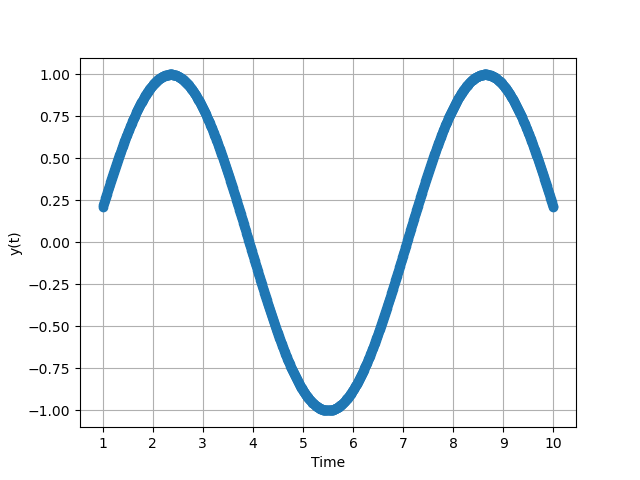
\includegraphics[width=1.0\linewidth]{figs/graph.png}
    \caption{plot of y(t)}
\end{figure}
\begin{align}
    G(s)&=\frac{1}{s+1}\\
    G(j\omega)&=\frac{1}{j\omega+1}\\
    |G(j\omega)|&=\frac{1}{\sqrt{\omega^2+1}}\\
    \angle G(j\omega)&=-tan^{-1}(\omega)
\end{align}
\begin{align}
    y(t)&=\sqrt{2}|G(j\omega_0)|_{\omega=\omega_0}sin(t-\angle G(j\omega_0)_{\omega=\omega_0})u(t)\\    
    \implies y(t)&=\sqrt{2}|G(j\omega)|_{\omega=1}sin(t-\angle G(j\omega)_{\omega=1})u(t)\\
    |G(j\omega)|_{\omega=1}&=\frac{1}{\sqrt{2}},\angle G(j\omega)_{\omega=1}=-45\degree\\
    y(t)&=\sqrt{2}\times\frac{1}{\sqrt{2}}sin(t-45\degree)u(t)\\
    y(t)&=sin(t-45\degree)u(t)
\end{align}
So,the amplitude of steady state output is 1
\end{document}
